\chapter{Estruturas}
\label{chapter:estruturas}

O subsistema estrutural ficou encarregado
de realizar a escolha de como obter uma cadeira de rodas e como realizar a fabricação da
transmissão para aumento do torque do motor para a roda.

Primeiramente, foi definido como seria feita a aquisição da cadeira de roda, se
seria manufaturada, comprada ou emprestada. Pelo curto período de
desenvolvimento de todo o projeto, e pelo fato dos componentes do grupo não
terem experiência com equipamentos de solda e modelagem de gabaritos para a
manufatura da estrutura, foi descartada a hipótese de construção da cadeira.
A segunda opção foi a estudada a possibilidade de comprar uma cadeira de roda,
porém não houve possibilidade de arrecadar fundos para esse investimento e pelo
tempo não houve a captação de investidores para o projeto. Por fim, com o
auxílio do Prof. Rhander Viana foi obtida uma cadeira de rodas do Hospital
Universitário de Brasília (HUB) onde foi emprestada uma cadeira de roda
Jaguaribe 1009. Ao fim do projeto, a cadeira de rodas será devolvida ao hospital.

O segundo ponto principal destinado a estrutura, foi a escolha de um tipo de
transmissão para realizar a movimentação da cadeira. Em conjunto com o
subsistema de controle e alimentação a forma escolhida para transmitir o torque do motor
para a cadeira foi a utilização de um disco de atrito que fica em contato com a
roda. Foi escolhida esta maneira para transmissão pelo fato de manufaturar uma
caixa de redução para o motor seria algo que não teria tempo hábil, ou seria
algo fora dos padrões orçamentários do projeto.

\section{Estrutura da Cadeira de Rodas}

Como explicado anteriormente, foi escolhida a aquisição de uma cadeira junto ao
Hospital Universitário de Brasília, onde foi realizado o empréstimo da cadeira
até o fim do projeto. A cadeira é a Cadeira de Rodas Jaguaribe 1009, como mostra
 a Figura \ref{fig:original_chair} abaixo.

\begin{figure}[!htb]
    \begin{center}
        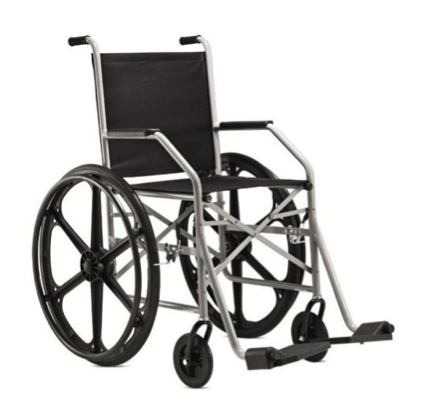
\includegraphics{figuras/original_chair.png}
    \end{center}
    \caption{Cadeira de Rodas Jaguaribe 1009.}
    \label{fig:original_chair}
\end{figure}

Esta cadeira é composta de uma estrutura metálica de aço carbono 1009, que
possui características de ser mais leve e suporta normalmente 90kg. O assento
e o encosto traseiro são constituídos de courvim, um tipo de tecido muito
utilizado para este fim.

A cadeira adquirida pelo grupo tinha algumas avarias, como rodas empenadas,
alguns aros das rodas faltando, tecido de courvim do assento e do encosto
rasgados e câmara de ar dos pneus rompidas. Foi necessário fazer a desempenagem
das rodas, troca da câmara de ar dos pneus, e compra dos aros para ter uma
cadeira em perfeito estado.

Como não foi necessário a manufatura da cadeira, apenas realizamos a modelagem
da cadeira de rodas em ambiente CAD para ter uma primeira impressão das
modificações necessárias. Como o escopo do projeto abrange
uma cadeira de rodas motorizada, que realiza monitoramentos de saúde do usuário, a
cadeira teria que possuir alguns detalhes na estrutura. A cadeira modelada em
ambiente CAD é apresentada na Figura \ref{fig:first_cad_chair}.

\begin{figure}[!htb]
    \begin{center}
        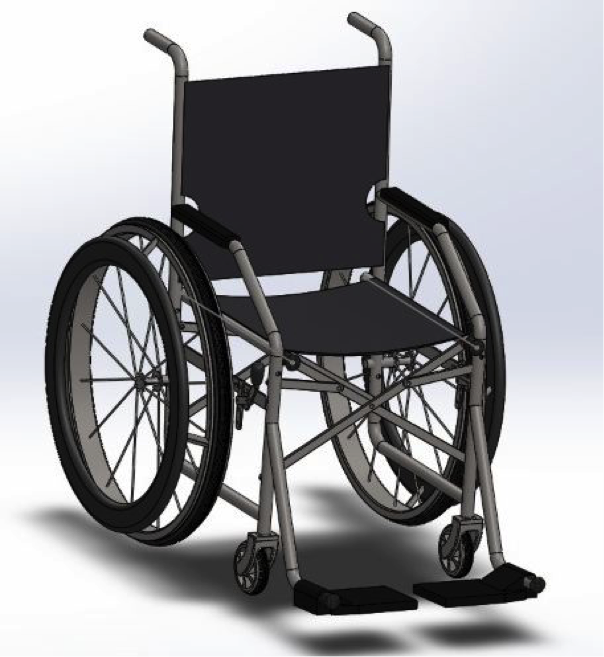
\includegraphics{figuras/first_cad_chair.png}
    \end{center}
    \caption{Desenho em ambiente CAD da Cadeira de Rodas.}
    \label{fig:first_cad_chair}
\end{figure}

Na Figura \ref{fig:first_cad_chair} é possível perceber a inserção do disco de
atrito no projeto, para realização do papel da transmissão, utilização de uma
placa para suportar o disco de atrito e o motor, além da gaveta para suportar o
peso e tornar de fácil remoção para recarga a bateria.

\section{Análises assistidas por Computador (CAD/CAE)}

Antes de manufaturar, houve um estudo minucioso em relação à como a estrutura
se comportaria em relação as cargas que são inseridas no sistema. Como a
cadeira já é planejada para suportar 90kg, e por ser um produto de grande
escala já é feito as análises estáticas, modal e de fadiga da mesma na própria
indústria para validar o projeto. Porém, como será adicionado parâmetros que
não são de fábrica, serão feitas análises tanto estática quanto modal na
cadeira para ter o projeto possuir confiabilidade. A análise estática é
utilizada para identificar tanto as deformações como as tensões que a estrutura
sofre quando exercida uma força. No projeto, foi utilizado o Software Solid
Works para fazer a análise, os parâmetros de estudo foram a Tensão de Von Mises
e Deformação de Von Mises. Assim para a estrutura ser aceita, é necessário que
a mesma tenha valores de tensão e deformação que não cause dano à estrutura,
neste caso não atinja a tensão de escoamento do material. A cadeira de roda
como citado anteriormente é constituída de aço carbono 1009, onde é composto
por 0,09\% de carbono, sendo assim um aço muito dúctil com baixa tensão de
escoamento, no caso 170MPa. Porém, como o Solid Works possui uma lista de
materiais reduzida, onde a tensão de escoamento mais próxima da usada na
cadeira é de 180MPa, com o aço 1010, que é muito parecido com o 1009, sendo
assim, para a análise estática será usado este material.
A Figura \ref{fig:static_analisys} demonstra os dados obtidos com a análise.

\begin{figure}[!htb]
    \begin{center}
        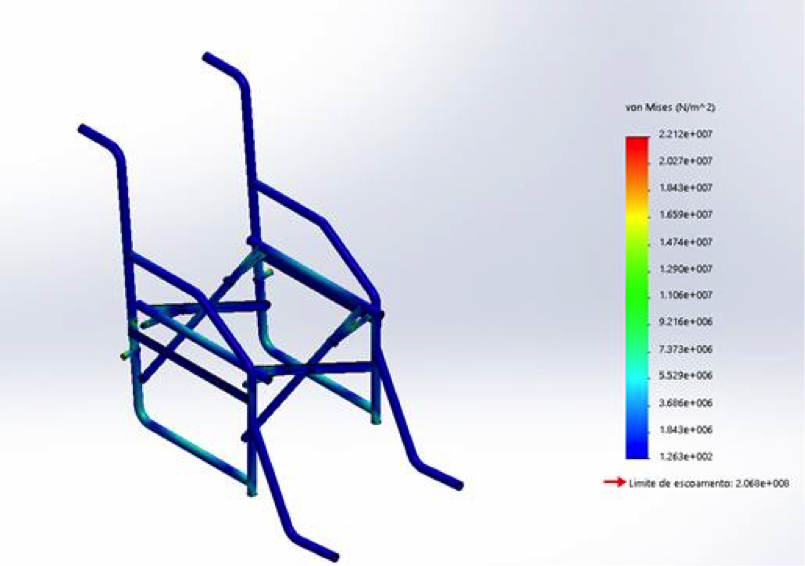
\includegraphics{figuras/static_analisys.png}
    \end{center}
    \caption{Análise Estática da Cadeira de Roda.}
    \label{fig:static_analisys}
\end{figure}

Na análise foi omitido diversos pontos, para que a análise fosse mais rápida,
porém todas as estruturas que foram removidas foram levada em consideração,
para isso estes componentes foram substituídos por forças.

Como pode ser visto na Figura \ref{fig:static_analisys}, a tensão máxima que ocorre na estrutura é de
221MPa, ou seja, a estrutura escoou, no caso passou do regime elástico para o
plástico. Porém, como pode ser visto também onde há a maior tensão de escoamento
são em pontos muito próximos ou quase nos apoios, ou seja, a teoria de mecânica
dos sólidos nos trás que uma carga no apoio não causa deformação, sendo assim,
será descartado os valores nos apoios, assim sobrando valores entre 92 e
129MPa, ou seja, validando o projeto.

Para a Análise Modal, foi ensaiado também no Solid Works, esta análise tem como
objetivo entregar ao usuário as frequências naturais que o produto tem,
ou seja, as frequências que a cadeira não pode ser excitada. A análise modal
funciona da seguinte forma, a peça é deixada sem apoios, e assim sofre uma
excitação, de acordo com a frequência de resposta da peça temos os valores da
frequência natural. Como possuímos 2 motores, que excitam a cadeira a 3 Hz
aproximadamente, é necessário que a cadeira tenha frequências naturais maiores
ou menores que este valor, caso contrário o projeto pode entrar em colapso.
Com as análises feitas no Software, obtivemos os seguintes valores:

\begin{table}[!htbp]
    \centering
    \caption{Valores da Análise Modal.}
    \label{tab:modal_analisys_values}
        \begin{tabular}{|l|l|l|}
            \hline
            \textbf{Número da frequência} & \textbf{Rad/s} & \textbf{Hertz} \\
            \hline
            1 & 0 & 0 \\
            \hline
            2 & 0 & 0 \\
            \hline
            3 & 0 & 0 \\
            \hline
            4 & 0.0028431 & 0.00045249 \\
            \hline
            5 & 0.0063894 & 0.0010169 \\
            \hline
            6 & 0.010349 & 0.0016472 \\
            \hline
            7 & 0.1351 & 0.021501 \\
            \hline
            8 & 0.17398 & 0.02769 \\
            \hline
            9 & 311.96 & 49.65 \\
            \hline
            10 & 342.36 & 54.488 \\
            \hline

        \end{tabular}
\end{table}

Os modos de frequência, que estão situados na primeira coluna condizem com os
modos em que o produto foi excitado, os valores de 1 até 6 deram muito próximo
de 0 pelo fato destes modos serem de translação e rotação. A partir do 7 já
existem frequências consideráveis, assim sendo estas que serão consideradas.
Como a frequência de trabalho é de 3Hz, temos que as frequências estão longe de
alcançar este ponto, a menos que exista algum problema de desalinhamento ou
desbalanceamento.

\section{Processo de Fabricação das Peças}

Para a manufatura do disco de atrito, foi necessário a utilização de técnicas de
processos de fabricação e conformação mecânica. Para a realização desta etapa
foi necessário a compra de um tarugo de alumínio que seria capaz de produzir
dois discos, um para cada roda. Todo o processamento do produto foi realizado
no Galpão da Universidade de Brasília Campus Gama, com o auxílio dos Técnicos
de Máquinas do local. Para a usinagem do tarugo foi necessário utilização do
torno para realizar os rebaixos necessários, foi utilizado também  uma técnica
de conformação mecânica que tornava a superfície do disco áspera, fazendo com
que a mesma obtivesse o coeficiente de atrito necessário para realização do
movimento da cadeira. Após esta conformação, foi realizado o corte do disco e a
usinagem dos furos necessários para a utilização do disco. Nesta etapa foi
furado na furadeira de bancada com uma broca com diâmetro praticamente igual ao
do eixo do motor, para haver uma conexão com interferência. Além da fabricação
de um furo para a passagem de um parafuso mosca, além da manufatura das roscas
para entrada do parafuso. que tem como função o melhor travamento entre o eixo
do motor e o disco de atrito. Na Figura \ref{fig:drawing_disc} temos o Desenho técnico do disco de
atrito.

\begin{figure}
    \begin{center}
        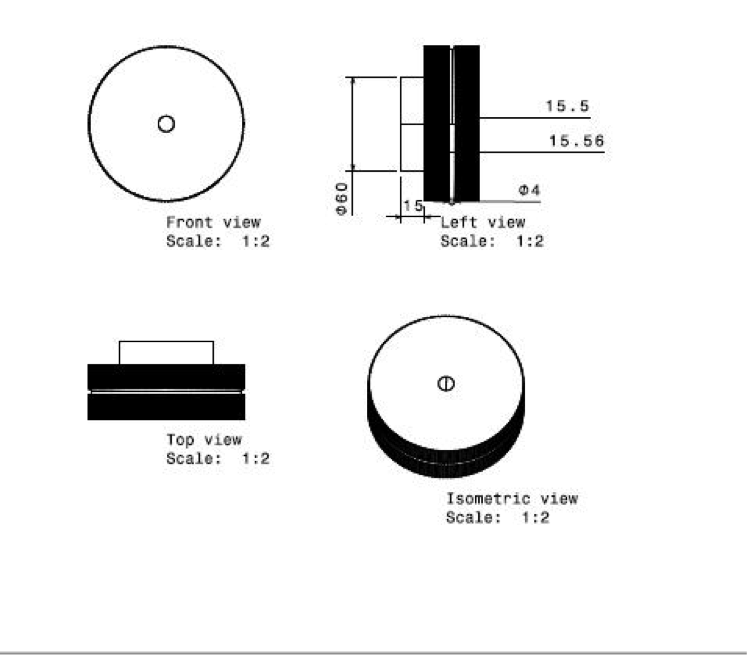
\includegraphics{figuras/drawing_disc.png}
    \end{center}
    \caption{Desenho técnico disco de atrito.}
    \label{fig:drawing_disc}
\end{figure}

Após o término do disco, foi manufaturada a placa que faz o suporte e fixação
entre o eixo do motor, disco de atrito e a cadeira de roda. Para conseguir uma
geometria que encaixasse com de maneira ótima, foi necessário fazer um gabarito
de um material que fosse de fácil usinagem, no caso o material escolhido foi o
MDF. Com o auxílio do motor, foi feito os furos na furadeira de bancada de
acordo com os furos do motor, onde eram feitos testes imediatamente após o furo
para ter certeza do tamanho do furo e de sua posição. Depois de encontrar um
padrão para a peça, foi usinada uma chapa de aço onde a mesma foi furada e
esmerilhada para chegar à geometria padrão. Os passos foram replicados para os
dois motores. A Figura \ref{fig:support_plate} demonstra o desenho técnico da
placa de suporte.

\begin{figure}
    \begin{center}
        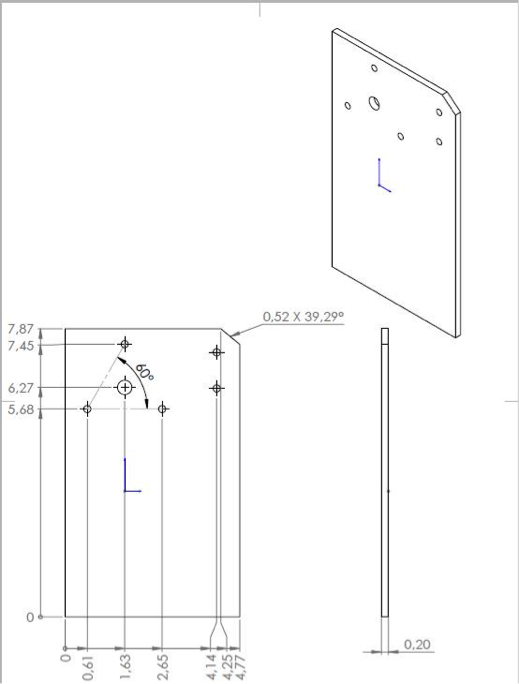
\includegraphics[scale=0.8]{figuras/support_plate.png}
    \end{center}
    \caption{Desenho Técnico da placa de suporte do motor e do disco de atrito}
    \label{fig:support_plate}
\end{figure}

Para não ser necessário mexer na estrutura da cadeira, foi decidido em amassar
o freio da cadeira de roda, de maneira que ele sirva de apoio, onde fizemos
furos para acoplar a placa que suporta o eixo. Desta forma, a cadeira irá poder
trabalhar tanto no manual quanto no automático, pelo fato do freio da cadeira
movimentar a placa e o disco de atrito. Esta foi uma das inúmeras preocupações,
tendo em vista que teria que existir um contato significativo entre o pneu e o
disco de atrito, por isso foram feitos vários testes em relação à posição da
placa, para ter a certeza de que a cadeira irá funcionar das duas formas.

Assim, a cadeira neste momento está disposta da seguinte forma, como mostra a
Figura \ref{fig:actual_state}.

\begin{figure}
    \begin{center}
        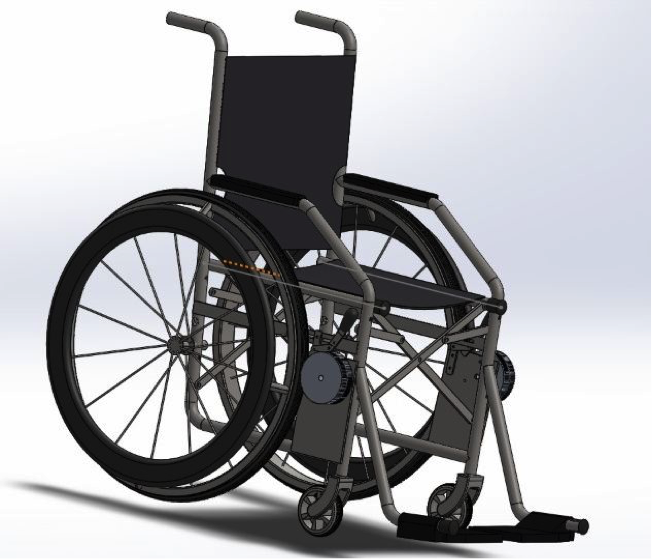
\includegraphics[scale=0.5]{figuras/actual_state.png}
    \end{center}
    \caption{Desenho do estado atual da Cadeira de Roda.}
    \label{fig:actual_state}
\end{figure}
